% ==================================
%
% PFC FRANCISCO SANCHEZ ARROYO
%
%===================================

\documentclass[a4paper,12pt,titlepage]{article}
\usepackage[includehead,includefoot]{geometry}
\geometry{left=2.5cm,right=2.5cm,top=2cm,bottom=2cm}
\usepackage{graphicx}
\usepackage[utf8]{inputenc} % Caracteres con acentos. 
\usepackage{longtable}
%\usepackage[spanish]{babel}
\usepackage{latexsym}
\usepackage{fancyhdr}
\usepackage{amsmath}
\usepackage{tabulary}
\usepackage{amssymb}
\usepackage{rotating} %rotar tablas y mas
\usepackage{hyperref}
% Poner colorlinks=false para la version impresa
\hypersetup{colorlinks=false, linkcolor=red,citecolor=green,filecolor=magenta,urlcolor=cyan}
%\usepackage{eurosym}
\usepackage{titlepic} %imagenes en la portada
\usepackage{lettrine}
\usepackage{booktabs} \usepackage{tabulary} %Para ajustar anchos de tablas
%% Cambia el formato de las cabeceras de las tablas y figuras
%\usepackage[small,normal,bf,up]{caption2}
%\renewcommand{\captionfont}{\small\itshape}
\usepackage{verbatim}
\usepackage{smartdiagram}
\usesmartdiagramlibrary{additions} 
\usepackage{tikz}
\usetikzlibrary{shapes}
%\usepackage[active,tightpage,floats]{preview}
%\setlength\PreviewBorder{5pt}%

%\titlepic{\includegraphics[width=12cm]{storefront.pdf}}
\title{Fabricating Labs\\
\Huge \textbf{Guidelines for designing and planning Fab Labs, Makerspaces and Innovation Facilities}}
\author{
by Francisco Sanchez Arroyo\\
The (Fabulous) Beach Lab
}
\date{Barcelona. \today}

%=====================================================
%=====================================================
\begin{document}

%\renewcommand{\tablename}{Taula}
%\renewcommand{\figurename}{Figura}
%\renewcommand{\listtablename}{Index de Taules}

% Values for plots
\newcommand{\D}{6} % number of dimensions (config option)
\newcommand{\U}{5} % number of scale units (config option)

\newdimen\R % maximal diagram radius (config option)
\R=3.5cm 
\newdimen\L % radius to put dimension labels (config option)
\L=4.3cm
% end values for plots


\newcommand{\A}{360/\D} % calculated angle between dimension axes  

\maketitle

\tableofcontents % Tabla de contenido
\clearpage
%\pagenumbering{roman}


%\addtocontents{toc}{\hfill Page \endgraf}
%\addtocontents{toc}{\bfseries Agradecimientos\endgraf}%
%\newpage
%\listoffigures % Índice de figuras
%\newpage 
%\listoftables % Índice de tablas 
%\newpage

\pagenumbering{arabic}



% Estilo de Cabecera y pie de pagina
\pagestyle{fancy}
\rhead{\textit{\textbf{Fabricating Labs}}}
\lhead{\textit{Guidelines for designing and planning of Innovation Spaces}}
\cfoot{-Page \thepage -}

\section*{About the author}
My name is Francisco Sanchez Arroyo, I am a MSc.Civil Engineer with specialty in Structural Engineering by the Polytechnic University of Catalonia. I am also an accredited LEED AP in Building Design and Construction by the GBCI, Fab Academy graduate and Bio Academy graduate. In late 2012 I quit my Real Estate job to focus in the maker movement and stablish my own innovation space, The Beach Lab. Passionate about education, technology, innovation and the environment, I balance my global citizenship with the love of my 2 beloved sons. Please feel free to reach me with any questions or comments about any of these topics.\\

\noindent{\url{hola@beachlab.org}}\\
\noindent{\url{http://beachlab.org}}\\
\noindent{\url{https://www.linkedin.com/in/fsancheza}}

\section*{License}
This work is licensed under Creative Commons Attribution ShareAlike 4.0 International License (CC BY-SA 4.0). 

\section*{Disclaimer}
This guide is work in progress, check the build date at the cover page. It is not yet complete and might contain missing and/or incorrect information. Handle with care.
\clearpage
\section{Introduction}
Are you planning to set up a Fab Lab or Makerspace? A common mistake is starting by placing machines and then figuring out the rest later. But did you think about the workflow around each machine? Are the other uses inside that room compatible with your process?  This Guide is intended to help identifying those workflows, cover the basic requirements and to avoid having future problems related to inadequate planning.\\

As a member of a global network of interconnected labs, I have had the opportunity to
visit, set up, fix and operate many fab labs all around the world, including mine, The Beach Lab. I not
only help fab labs to streamline the setup, operation and training of their facilities. I also
guide them to create better spaces that are not just rooms with a bunch of equipment, but
promote the development of a strong sharing community and interaction of its members.\\

While this document will need to be further
developed, it will settle the foundations for the work to be elaborated in your planning process.



\section{The Ideal Layout}
Many times I receive this question: \textit{What is the ideal Fab Lab layout?}
\subsection{The short answer} 
It does not exist such a thing.

\subsection{The long answer}
There is not and ideal layout for a Fab Lab. Every fab lab has its owns singularities that make
them unique spaces. But what makes all fab labs so great orbits around a very simple idea that
is represented in the three men holding each one shoulder in Fab Lab logo. \textit{Fab Labs are
places to learn, to make and to share}. 

\begin{figure}[h] %  figure placement: here, top, bottom
   \centering
   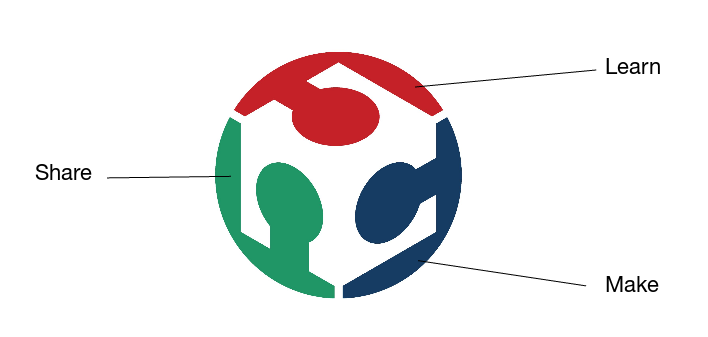
\includegraphics[width=8cm]{files/learn-make-share} 
\end{figure}

And these three values, should have a representation in the layout. Other desirable values to foster through the layout:
\begin{description}
\item[Flexibility.] The spaces should serve many purposes. A flexible design can virtually multiply
the space in your lab, making it suitable for many different activities. I was glad to see some
furniture and machines on wheels. It also requires incorporating hanging power cords, open
ceilings and flexible ducts for lasers exhausts.
\item[Modularity.] The space should be able to grow or shrink as the needs of the lab progresses.
\item[Sustainability.] This is a key and fundamental concept that it's behind the origin of fab labs.
\item[Sharing and collaboration.] The spaces we create should encourage people to cooperate
together.
\end{description}
 
\section{The Planning Process}
\subsection{Planning Phases}
\begin{description}
\item [Phase 1:] List the capabilities you would like to have in the Fab Lab. Elaborate your inventory according to your budget. This is a important step because you don't want to end up with duplicated equipment, missing equipment/materials, materials of doubtful utility and unbalanced number of machines.

\item [Phase 2:] Analyze the needs of these machines and their hosting spaces in terms of MEP (Mechanical, electrical,plumbing) and HSE (health, safety and environment). Determine which are the rooms that are
more suitable for each type of machine.
\item [Phase 3:] Determine a layout plan for the separation of the spaces.
\item [Phase 4:] Elaborate a plan to implement furniture, MEP and HSE needs.
\item [Phase 5:] Develop and execute the chosen solution.

\end{description}




\subsection{List of requirements to be assessed}
For each of the above levels of assessment we will identify the following requirements:
\begin{description}
\item [Operational Logistics:] How will the assets and people flow in, out and around? How will you manage the inventory (including maintenance, storage and locking requirements)? How will you control access? What's the maintenance plan? Is the facility ready for redundancy and resiliency when some equipment fail?

\item [Mechanical, Electrical and Plumbing (MEP) requirements:] Under this category it is included lighting requirements, HVAC systems, piping and plumbing, power and electrical requirements. Paying special attention to using the natural resources (natural lighting, natural ventilation, etc.) that can lower the environmental footprint of the facility.

\item [Health, Safety and Environment (HSE):] We should take very seriously Health, Safety and Environment aspects in Fab Labs. It's our social responsibility and our legacy to take care of the users, faculty and employees.
The inventory of equipment, materials, workflows and processes that Fab Labs use and recommend have been
carefully selected in order to comply with the highest standards of HSE. This also includes ergonomy and waste management.
\end{description}

\subsection{Levels of assessment}
When planning a Fab Lab, the above requirements should be assessed in 4 levels of detail:
\begin{itemize}
\item \textbf{The machine or process}. Each machine and process has its owns requirements.
\item \textbf{The workflow around that machine or process}. A machine it's usually part of a bigger process or workflow, whose requirements you need to analyse too. If workflows
are not identified, machines and materials will be  placed randomly (incorrectly) placed without a
logical arrangement. Ideally every machine and process should follow a logic workflow and
have all its materials, inflows and outflows at reaching distance.

\item \textbf{The room containing that workflow} must be analysed specially looking for incompatibilities regarding noise, dust, ventilation, etc. Not only Learning, making and sharing spaces should be separated. Within the making
area of the lab, there should be separation of clean and quiet with loud and messy areas to avoid incompatible uses colliding.
\item \textbf{The building containing that room} must be assessed as well. High frecuency vibrations created by digital fabrication machines can travel through the structure of the building causing trouble in areas very far areas from its origin.
\end{itemize}

\clearpage
  
\section{Processes and Workflows found in a Fab Lab}

\subsection{Vinyl Cutting}
\begin{figure}[h]

\centering
\smartdiagramset{
    set color list={red!10, red!25,red!40, red!55},
    sequence item border color=black,
    sequence item text color=black,
    sequence item border size=1.2\pgflinewidth,
    sequence item font size=\scriptsize\sffamily,
    additions={
        additional item shape=rectangle,
        additional item fill color=gray!20,
        additional item border color=black,
        additional arrow line width=2pt,
        additional arrow tip=to,
        additional arrow color=black,
        additional item font=\scriptsize\sffamily,
      }
}
\smartdiagramadd[sequence diagram]{Materials (1),Machine (2) \\ Roland GX 24, Postprocess\\ (3), Waste (4)}
{below of sequence-item1/{Raw and scrap material},below of sequence-item2/Reusable Scrap}
\smartdiagramconnect{to-}{sequence-item1/additional-module1}
\smartdiagramconnect{-to}{sequence-item2/additional-module2}
\vspace{1cm}
\end{figure}
\subsubsection*{Notes}
\begin{itemize}
\item (1) Additional items: X-acto, scissors, masking tape, vinyl gloves
\item (2) This area requires also space for a computer for design and operation tasks. Provide enough power plugs (minimum 3)
\item (2) The back of the machine must be reachable
\item (2) Additional items: Tweezers, X-acto, scissors
\item (3) This area requires the witdh of the biggest roll that the machine can handle and plenty of light
\item (3) Additional items: Tweezers, X-acto, scissors
\item (4) Waste: Paper backing, vinyl, Copper film, epoxy film.
\end{itemize}
\subsubsection*{Risks}
\begin{itemize}
\item Hand trapped by machine movement
\item Cuts with sharp objects
\end{itemize}
\subsubsection*{Personal Protective Elements (PPE)}
\begin{itemize}
\item None required
\end{itemize}
\clearpage

\subsection{3D Printing FDS}
\begin{figure}[h]

\centering
\smartdiagramset{
    set color list={red!10, red!25,red!40, red!55},
    sequence item border color=black,
    sequence item text color=black,
    sequence item border size=1.2\pgflinewidth,
    sequence item font size=\scriptsize\sffamily,
    additions={
        additional item shape=rectangle,
        additional item fill color=gray!20,
        additional item border color=black,
        additional arrow line width=2pt,
        additional arrow tip=to,
        additional arrow color=black,
        additional item font=\scriptsize\sffamily,
      }
}
\smartdiagramadd[sequence diagram]{Materials (1),Machine (2) \\ 3D printer, Postprocess\\ (3), Waste (4)}
{below of sequence-item1/Filament}
\smartdiagramconnect{to-}{sequence-item1/additional-module1}
\vspace{1cm}
\end{figure}
\subsubsection*{Notes}
\begin{itemize}
\item (1) Filaments require low moisture environment
\item (3) Additional items: Wire cutter, spatula
\item (2) Machine requires rear inspection
\item (2) Power requirements: Most 3D printers don't require a computer. Newest require network connection.
\item (2) HVAC direct airflow or low room temperature might affect buildplate adhesion and layer cooling
\item (3) Additional items: X-acto, pliers, wire cutter
\item (4) PLA and ABS based plastics
\end{itemize}
\subsubsection*{Risks}
\begin{itemize}
\item Hand trapped by machine movement
\item Burn by noozle or buildplate
\item Hot plastic splatters caused by moisture inside filament
\end{itemize}
\subsubsection*{Personal Protective Elements (PPE)}
\begin{itemize}
\item Eye protection is recommended for kids
\end{itemize}
\clearpage


\subsection{Laser Cutting}
\begin{figure}[h]

\centering
\smartdiagramset{
    set color list={red!10, red!25,red!40, red!55},
    sequence item border color=black,
    sequence item text color=black,
    sequence item border size=1.2\pgflinewidth,
    sequence item font size=\scriptsize\sffamily,
    additions={
        additional item shape=rectangle,
        additional item fill color=gray!20,
        additional item border color=black,
        additional arrow line width=2pt,
        additional arrow tip=to,
        additional arrow color=black,
        additional item font=\scriptsize\sffamily,
      }
}
\smartdiagramadd[sequence diagram]{Materials (1),Machine (2) \\ Laser Cutter, Postprocess\\ (3), Waste (4)}
{below of sequence-item1/{Raw and scrap material},below of sequence-item2/Reusable Scrap}
\smartdiagramconnect{to-}{sequence-item1/additional-module1}
\smartdiagramconnect{-to}{sequence-item2/additional-module2}
\vspace{1cm}
\end{figure}
\subsubsection*{Notes}
\begin{itemize}
\item (1) Maintaining order of scrap material is important
\item (1) Cardboard and wood are sensitive to moisture
\item (2) The room requires ventilation and air renovation from exterior
\item (2) The laser is usually a noisy environment, specially if there is also a filter installed
\item (2) It is required also space for computer for design and operation of the laser
\item (2) Power requirements: Provide at least 6 power plugs
\item (3) Clean up scrap material and store it in (1)
\item (4) Cardboard, wood, plastics
\end{itemize}
\subsubsection*{Risks}
\begin{itemize}
\item Health issues due to long-term exposure to fumes 
\item Cuts by sharp edges of material
\end{itemize}
\subsubsection*{Personal Protective Elements (PPE)}
\begin{itemize}
\item Recommended gloves for handling material and scrap
\end{itemize}
\clearpage


\subsection{Electronics Production}
\begin{figure}[h]
\centering
\smartdiagramset{
    set color list={red!10, red!25,red!40, red!55, red!70},
    sequence item border color=black,
    sequence item text color=black,
    sequence item border size=1.2\pgflinewidth,
    sequence item font size=\scriptsize\sffamily,
    additions={
        additional item shape=rectangle,
        additional item fill color=gray!20,
        additional item border color=black,
        additional arrow line width=2pt,
        additional arrow tip=to,
        additional arrow color=black,
        additional item font=\scriptsize\sffamily,
      }
}
\smartdiagramadd[sequence diagram]{Design (1),Machine (2) \\ SRM 20, Stuff (3), Test (4),Waste (5)}
{below of sequence-item2/{FR1 boards and milling bits},below of sequence-item3/Electronic components}
\smartdiagramconnect{to-}{sequence-item2/additional-module1}
\smartdiagramconnect{to-}{sequence-item3/additional-module2}
\vspace{1cm}
\end{figure}
\subsubsection*{Notes}
\begin{itemize}
\item (1) Area for a computer next to the machine for design and machine operation. 3 power plugs
\item (2) Additional items: Spatula, double-side tape, X-acto, Allen keys for milling bits, magnets
\item (3) As this usually becomes a bottleneck of the process a minimum of 2 seats for soldering operators should be plannned
\item (3) Easily accessible cabinets with electronic components
\item (3) This area requires ventilation and air renovation, plenty of light and magnifying equipment
\item (3) Power requirements for 2 seats: 6 plugs
\item (4) 2 seats area for power supply, oscilloscope and function generator. Power requirements 6 plugs
\item (5) Waste: Paper dust, FR1 boards, broken bits, electronic components
\end{itemize}
\subsubsection*{Risks}
\begin{itemize}
\item Fumes inhalation
\item Electric shock
\item Cuts by sharp objects
\item Burns by soldering iron
\end{itemize}
\subsubsection*{Personal Protective Elements (PPE)}
\begin{itemize}
\item Gloves for removing boards and soldering
\item Eye protection for soldering
\item Isolating shoes
\end{itemize}
\clearpage


\subsection{Molding and Casting}
Molding and casting is a 3-phase process that can be done at different time and in separated rooms
\begin{figure}[h]

\centering
\smartdiagramset{
    set color list={red!10, red!25,red!40, red!55},
    sequence item border color=black,
    sequence item text color=black,
    sequence item border size=1.2\pgflinewidth,
    sequence item font size=\scriptsize\sffamily,
    additions={
        additional item shape=rectangle,
        additional item fill color=gray!20,
        additional item border color=black,
        additional arrow line width=2pt,
        additional arrow tip=to,
        additional arrow color=black,
        additional item font=\scriptsize\sffamily,
      }
}
\smartdiagramadd[sequence diagram]{Materials (1),Machine (2) \\ SRM 20}
{below of sequence-item1/{Machinable wax},below of sequence-item2/Reusable Wax chips}
\smartdiagramconnect{to-}{sequence-item1/additional-module1}
\smartdiagramconnect{-to}{sequence-item2/additional-module2}
\vspace{1cm}
\end{figure}

\begin{figure}[h]

\centering
\smartdiagramset{
    set color list={green!10, green!25,green!40},
    sequence item border color=black,
    sequence item text color=black,
    sequence item border size=1.2\pgflinewidth,
    sequence item font size=\scriptsize\sffamily,
    additions={
        additional item shape=rectangle,
        additional item fill color=gray!20,
        additional item border color=black,
        additional arrow line width=2pt,
        additional arrow tip=to,
        additional arrow color=black,
        additional item font=\scriptsize\sffamily,
      }
}
\smartdiagramadd[sequence diagram]{Preprocess (3),Molding (4), Waste (5)}
{below of sequence-item1/{Silicons and Rubbers},below of sequence-item2/Reusable Soft Mold}
\smartdiagramconnect{to-}{sequence-item1/additional-module1}
\smartdiagramconnect{-to}{sequence-item2/additional-module2}
\vspace{1cm}
\end{figure}

\begin{figure}[h]

\centering
\smartdiagramset{
    set color list={yellow!10, yellow!25,yellow!40},
    sequence item border color=black,
    sequence item text color=black,
    sequence item border size=1.2\pgflinewidth,
    sequence item font size=\scriptsize\sffamily,
    additions={
        additional item shape=rectangle,
        additional item fill color=gray!20,
        additional item border color=black,
        additional arrow line width=2pt,
        additional arrow tip=to,
        additional arrow color=black,
        additional item font=\scriptsize\sffamily,
      }
}
\smartdiagramadd[sequence diagram]{Preprocess (6),Casting (7), Waste (8)}
{below of sequence-item1/{Casting Materials}}
\smartdiagramconnect{to-}{sequence-item1/additional-module1}
\vspace{1cm}
\end{figure}

\subsubsection*{Notes}
\begin{itemize}
\item (1)(2) Phase 1 can be executed in the same room as electronics production. But it requires to clean and vacuum the machine and surrounding area prior to milling the wax. This phase produces virtually zero waste. A dedicated vacuum machine or a clean brush is recommended to pick up all the wax chips for future use.
\item Phase 2 and Phase 3 can be executed in a separate room. These phases require a ventilated area and access to water and a sink.
\item (3) Refer to MSDS for important health and safety information
\item (4) Store reusable molds in the same storage room as silicons
\item (5) Waste: Pots, gloves, sticks, etc, stained with silicons and rubbers
\item (8) Waste: Pots, gloves, sticks, etc, stained with casting materials
\end{itemize}
\subsubsection*{Risks}
\begin{itemize}
\item Inhalation of dangerous volatile substances
\item Eye, skin and lung irritation
\end{itemize}
\subsubsection*{Personal Protective Elements (PPE)}
\begin{itemize}
\item Lab coat, vinyl gloves and eye protection during the molding and casting phases
\item Masks and respirators upon the MSDS specs of the materials
\end{itemize}
\clearpage


\subsection{Composites}
Composites is a 2-phase process that can be done at different time and in separated rooms
\begin{figure}[h]

\centering
\smartdiagramset{
    set color list={red!10, red!25,red!40, red!55},
    sequence item border color=black,
    sequence item text color=black,
    sequence item border size=1.2\pgflinewidth,
    sequence item font size=\scriptsize\sffamily,
    additions={
        additional item shape=rectangle,
        additional item fill color=gray!20,
        additional item border color=black,
        additional arrow line width=2pt,
        additional arrow tip=to,
        additional arrow color=black,
        additional item font=\scriptsize\sffamily,
      }
}
\smartdiagramadd[sequence diagram]{Materials (1),Machine (2) \\ Shopbot, Waste (3)}
{below of sequence-item1/{High Density Foam}}
\smartdiagramconnect{to-}{sequence-item1/additional-module1}
\vspace{1cm}
\end{figure}

\begin{figure}[h]

\centering
\smartdiagramset{
    set color list={green!10, green!25,green!40},
    sequence item border color=black,
    sequence item text color=black,
    sequence item border size=1.2\pgflinewidth,
    sequence item font size=\scriptsize\sffamily,
    additions={
        additional item shape=rectangle,
        additional item fill color=gray!20,
        additional item border color=black,
        additional arrow line width=2pt,
        additional arrow tip=to,
        additional arrow color=black,
        additional item font=\scriptsize\sffamily,
      }
}
\smartdiagramadd[sequence diagram]{Preprocess (4),Composite Layout (5), Waste (6)}
{below of sequence-item1/{Fabrics and Resins},below of sequence-item2/Reusable Mold}
\smartdiagramconnect{to-}{sequence-item1/additional-module1}
\smartdiagramconnect{-to}{sequence-item2/additional-module2}
\vspace{1cm}
\end{figure}


\subsubsection*{Notes}
\begin{itemize}
\item (2) Room containing the Shopbot is a very noisy, dusty and dangerous environment. Recommended separate room.
\item (2) Room containing the Shopbot must have ventilation and filtration system. Refer to calculations in following sections.
\item (3) Waste: Foam dust, high density foam
\item (4) This phase requires a ventilated area and access to water and a sink
\item (5) Store reusable molds in (1)
\item (6) Waste: Sand paper and resin dust
\end{itemize}
\subsubsection*{Risks}
\begin{itemize}
\item Fine dust particles inhalation in milling phase
\item Fast spinning cutting tool in milling phase
\item Debris in milling phase
\item Noise damage
\item Being trapped by moving machine or spindle
\item Eye, skin and lung irritation due to resins
\end{itemize}
\subsubsection*{Personal Protective Elements (PPE)}
\begin{itemize}
\item Eye, ear protection
\item Appropriate gloves for handling materials
\item Coat, eye protection, gloves and mask/respirators during composite layout phase
\end{itemize}
\clearpage


\subsection{Large CNC}
\begin{figure}[h]

\centering
\smartdiagramset{
    set color list={red!10, red!25,red!40, red!55},
    sequence item border color=black,
    sequence item text color=black,
    sequence item border size=1.2\pgflinewidth,
    sequence item font size=\scriptsize\sffamily,
    additions={
        additional item shape=rectangle,
        additional item fill color=gray!20,
        additional item border color=black,
        additional arrow line width=2pt,
        additional arrow tip=to,
        additional arrow color=black,
        additional item font=\scriptsize\sffamily,
      }
}
\smartdiagramadd[sequence diagram]{Materials (1),Machine (2) \\ Shopbot, Waste (3)}
{below of sequence-item1/{Wood}}
\smartdiagramconnect{to-}{sequence-item1/additional-module1}
\vspace{1cm}
\end{figure}
\subsubsection*{Notes}
\begin{itemize}
\item (2) Room containing the Shopbot is a very noisy, dusty and dangerous environment. Recommended separate room.
\item (2) Room containing the Shopbot must have ventilation and filtration system. Refer to calculations in following sections.
\end{itemize}
\subsubsection*{Risks}
\begin{itemize}
\item Fine dust particles inhalation in milling phase
\item Fast spinning cutting tool in milling phase
\item Debris in milling phase
\item Being trapped by moving machine or spindle
\end{itemize}
\subsubsection*{Personal Protective Elements (PPE)}
\begin{itemize}
\item Eye, ear protection
\item Appropriate gloves for handling materials 
\end{itemize}

\subsubsection*{Filtration System}
Most of the time you are going to be working with wood materials. This equipment
produces a loud and dusty environment. So, the first advice is
placing all this equipment in a separated room. Most of these machines come with
a dust collector that will capture the thicker wood particles. But still there will be finer cloud
particles up to 10 micron that will not only float for around 30 minutes, but also will be
suspended again with the slightest movement of air. The fine dust becomes a serious health issue. These
fine particles will come from 2 sources. One is the dust collection felt bag that will allow
particles up to 3 microns to escape through the fabric. And the second source is particles that because their high speed will never enter the dust collection system.\\

So I suggest that you install in these rooms a filtration system rated so that it will cycle through
the entire volume of air in the room 6 to 8 times per hour. And with a timer for 2, 4, or 8 hours
so that when the user will walk out of the room will flip the switch and forget about it.


\section{Technical aspects}

\section{What's next?}


\end{document}
